\chapter{List, Hashtable, Stack, Heap, Sort}

\section{Add Two Numbers} %%%%%%%%%%%%%%%%%%%%%%



\subsubsection{Description}
You are given two non-empty linked lists representing two non-negative integers. The digits are stored in reverse order and each of their nodes contain a single digit. Add the two numbers and return it as a linked list.

You may assume the two numbers do not contain any leading zero, except the number 0 itself.

\textbf{Input:} \code{(2 -> 4 -> 3) + (5 -> 6 -> 4)}

\textbf{Output:} \code{7 -> 0 -> 8}

\subsubsection{Solution}

\begin{Code}
public ListNode addTwoNumbers(ListNode l1, ListNode l2) {
    ListNode dummy = new ListNode(0), cur = dummy;

    for (int carry = 0; l1 != null || l2 != null || carry > 0; ) {
        int n1 = l1 != null ? l1.val : 0;
        l1 = l1 != null ? l1.next : null;
        int n2 = l2 != null ? l2.val : 0;
        l2 = l2 != null ? l2.next : null;

        int sum = n1 + n2 + carry;
        ListNode node = new ListNode(sum % 10);
        carry = sum / 10;
        cur.next = node;
        cur = node;
    }

    return dummy.next;
}
\end{Code}

\newpage

\section{Add Two Numbers II} %%%%%%%%%%%%%%%%%%%%%%



\subsubsection{Description}
You are given two non-empty linked lists representing two non-negative integers. The most significant digit comes first and each of their nodes contain a single digit. Add the two numbers and return it as a linked list.

You may assume the two numbers do not contain any leading zero, except the number 0 itself.

\textbf{Follow up:}

What if you cannot modify the input lists? In other words, reversing the lists is not allowed.

\textbf{Example:}

\textbf{Input:} \code{(7 -> 2 -> 4 -> 3) + (5 -> 6 -> 4)}

\textbf{Output:} \code{7 -> 8 -> 0 -> 7}
\subsubsection{Solution}

\begin{Code}
public ListNode addTwoNumbers(ListNode l1, ListNode l2) {
    Stack<Integer> s1 = new Stack<Integer>();
    Stack<Integer> s2 = new Stack<Integer>();

    while (l1 != null) {
        s1.push(l1.val);
        l1 = l1.next;
    }
    ;
    while (l2 != null) {
        s2.push(l2.val);
        l2 = l2.next;
    }

    int sum = 0;
    ListNode list = new ListNode(0);
    while (!s1.empty() || !s2.empty()) {
        if (!s1.empty()) sum += s1.pop();
        if (!s2.empty()) sum += s2.pop();
        list.val = sum % 10;
        ListNode head = new ListNode(sum / 10);
        head.next = list;
        list = head;
        sum /= 10;
    }

    return list.val == 0 ? list.next : list;
}
\end{Code}

\newpage

\section{Reverse Linked List} %%%%%%%%%%%%%%%%%%%%%%



\subsubsection{Description}
Reverse a singly linked list.

\textbf{Hint:}

A linked list can be reversed either iteratively or recursively. Could you implement both?

\subsubsection{Solution I}

\begin{Code}
public ListNode reverseList(ListNode head) {
    if (head == null || head.next == null) {
        return head;
    }
    ListNode next = head.next;
    ListNode newHead = reverseList(next);
    next.next = head;
    head.next = null;
    return newHead;
}
\end{Code}

\subsubsection{Solution II}
\begin{Code}
// 耗时0ms
public ListNode reverseList2(ListNode head) {
    ListNode dummy = new ListNode(0);

    for (ListNode p = head; p != null; ) {
        ListNode next = p.next;
        p.next = dummy.next;
        dummy.next = p;
        p = next;
    }

    return dummy.next;
}
\end{Code}

\newpage

\section{Reverse Linked List II} %%%%%%%%%%%%%%%%%%%%%%



\subsubsection{Description}
Reverse a linked list from position m to n. Do it in-place and in one-pass.

For example:

Given \code{1->2->3->4->5->NULL}, m = 2 and n = 4,

return \code{1->4->3->2->5->NULL}.

\textbf{Note:}

Given m, n satisfy the following condition:

1 ≤ m ≤ n ≤ length of list.

\subsubsection{Solution}

\begin{Code}
public ListNode reverseBetween(ListNode head, int m, int n) {
    if (head == null) return null;
    ListNode dummy = new ListNode(0);
    dummy.next = head;
    ListNode pre = dummy;
    for (int i = 0; i < m - 1; i++) pre = pre.next;

    ListNode start = pre.next;
    ListNode then = start.next;

    for (int i = 0; i < n - m; i++) {
        start.next = then.next;
        then.next = pre.next;
        pre.next = then;
        then = start.next;
    }

    return dummy.next;
}
\end{Code}

\newpage

\section{Sort List} %%%%%%%%%%%%%%%%%%%%%%



\subsubsection{Description}
Sort a linked list in O(n log n) time using constant space complexity.

\subsubsection{Solution}

\begin{Code}
public ListNode sortList(ListNode head) {
    if (head == null || head.next == null)
        return head;

    ListNode prev = null, slow = head, fast = head;

    while (fast != null && fast.next != null) {
        prev = slow;
        slow = slow.next;
        fast = fast.next.next;
    }

    prev.next = null;
    ListNode l1 = sortList(head);
    ListNode l2 = sortList(slow);
    return merge(l1, l2);
}

ListNode merge(ListNode l1, ListNode l2) {
    ListNode l = new ListNode(0), p = l;

    while (l1 != null && l2 != null) {
        if (l1.val < l2.val) {
            p.next = l1;
            l1 = l1.next;
        } else {
            p.next = l2;
            l2 = l2.next;
        }
        p = p.next;
    }

    if (l1 != null)
        p.next = l1;

    if (l2 != null)
        p.next = l2;

    return l.next;
}
\end{Code}

\newpage

\section{Linked List Cycle} %%%%%%%%%%%%%%%%%%%%%%



\subsubsection{Description}
Given a linked list, determine if it has a cycle in it.

\textbf{Follow up:}

Can you solve it without using extra space?

\subsubsection{Solution}

\begin{Code}
public boolean hasCycle(ListNode head) {
    if (head == null) {
        return false;
    }

    ListNode fast = head.next, slow = head;

    for ( ; fast != null && fast.next != null; fast = fast.next.next, slow = slow.next) {
        if (fast == slow) {
            return true;
        }
    }

    return false;
}
\end{Code}

\newpage

\section{Linked List Cycle II} %%%%%%%%%%%%%%%%%%%%%%



\subsubsection{Description}
Given a linked list, return the node where the cycle begins. If there is no cycle, return null.

\textbf{Note:} Do not modify the linked list.

\textbf{Follow up:}

Can you solve it without using extra space?

\subsubsection{Solution}

\begin{Code}
public ListNode detectCycle(ListNode head) {
    if (head == null || head.next == null) return null;

    ListNode firstp = head;
    ListNode secondp = head;
    boolean isCycle = false;

    while (firstp != null && secondp != null) {
        firstp = firstp.next;
        if (secondp.next == null) return null;
        secondp = secondp.next.next;
        if (firstp == secondp) {
            isCycle = true;
            break;
        }
    }

    if (!isCycle) return null;
    firstp = head;
    while (firstp != secondp) {
        firstp = firstp.next;
        secondp = secondp.next;
    }

    return firstp;
}
\end{Code}

\newpage

\section{Odd Even Linked List} %%%%%%%%%%%%%%%%%%%%%%



\subsubsection{Description}
Given a singly linked list, group all odd nodes together followed by the even nodes. Please note here we are talking about the node number and not the value in the nodes.

You should try to do it in place. The program should run in O(1) space complexity and O(nodes) time complexity.

\textbf{Example:}
\begin{Code}
Given 1->2->3->4->5->NULL,
return 1->3->5->2->4->NULL.
\end{Code}

\textbf{Note:}

The relative order inside both the even and odd groups should remain as it was in the input.

The first node is considered odd, the second node even and so on ...

\subsubsection{Solution}

\begin{Code}
public ListNode oddEvenList(ListNode head) {
    ListNode odd = new ListNode(0), pOdd = odd;
    ListNode even = new ListNode(0), pEven = even;

    int index = 1;
    for (ListNode p = head; p != null; p = p.next) {
        if ((index++ & 1) > 0) {
            pOdd.next = p;
            pOdd = pOdd.next;
        } else {
            pEven.next = p;
            pEven = pEven.next;
        }
    }

    pOdd.next = null;
    pEven.next = null;

    pOdd.next = even.next;
    return odd.next;
}
\end{Code}

\newpage

\section{Merge Two Sorted Lists} %%%%%%%%%%%%%%%%%%%%%%



\subsubsection{Description}
Merge two sorted linked lists and return it as a new list. The new list should be made by splicing together the nodes of the first two lists.

\subsubsection{Solution}

\begin{Code}
// 耗时15ms
public ListNode mergeTwoLists(ListNode l1, ListNode l2) {
    ListNode dummy = new ListNode(0);
    ListNode p = l1, q = l2, cur = dummy;
    for ( ; p != null && q != null; ) {
        if (p.val < q.val) {
            cur.next = p;
            p = p.next;
        } else {
            cur.next = q;
            q = q.next;
        }
        cur = cur.next;
    }
    cur.next = p != null ? p : q;
    return dummy.next;
}
\end{Code}

\newpage

\section{Merge k Sorted Lists} %%%%%%%%%%%%%%%%%%%%%%



\subsubsection{Description}
Merge k sorted linked lists and return it as one sorted list. Analyze and describe its complexity.

\subsubsection{Solution}

\begin{Code}
/**
 * 这里要注意lists中可能有node为null
 */
public ListNode mergeKLists(ListNode[] lists) {
    ListNode dummy = new ListNode(0), cur = dummy;

    PriorityQueue<ListNode> queue = new PriorityQueue<>(new Comparator<ListNode>() {
        @Override
        public int compare(ListNode node1, ListNode node2) {
            if (node1.val == node2.val) {
                return 0;
            } else if (node1.val < node2.val) {
                return -1;
            } else {
                return 1;
            }
        }
    });

    for (ListNode node : lists) {
        if (node != null) {
            queue.offer(node);
        }
    }

    while (!queue.isEmpty()) {
        ListNode node = queue.poll();
        cur.next = node;
        cur = cur.next;
        if (node.next != null) {
            queue.offer(node.next);
        }
    }

    return dummy.next;
}
\end{Code}

\newpage

\section{Intersection of Two Linked Lists} %%%%%%%%%%%%%%%%%%%%%%



\subsubsection{Description}
Write a program to find the node at which the intersection of two singly linked lists begins.

For example, the following two linked lists:
\begin{Code}
A:          a1 → a2
                   ↘
                     c1 → c2 → c3
                   ↗
B:     b1 → b2 → b3
\end{Code}

begin to intersect at node c1.


\textbf{Notes:}

If the two linked lists have no intersection at all, return null.

The linked lists must retain their original structure after the function returns.

You may assume there are no cycles anywhere in the entire linked structure.

Your code should preferably run in O(n) time and use only O(1) memory.
\subsubsection{Solution}

\begin{Code}
public ListNode getIntersectionNode(ListNode headA, ListNode headB) {
    int lenA = 0, lenB = 0;
    for (ListNode p = headA; p != null; p = p.next, lenA++);
    for (ListNode p = headB; p != null; p = p.next, lenB++);
    ListNode p = lenA > lenB ? headA : headB;
    ListNode q = lenA > lenB ? headB : headA;
    for (int i = 0; i < Math.abs(lenA - lenB); i++, p = p.next);
    for ( ; p != null && q != null; p = p.next, q = q.next) {
        if (p == q) {
            return p;
        }
    }
    return null;
}
\end{Code}

\newpage

\section{Copy List with Random Pointer} %%%%%%%%%%%%%%%%%%%%%%



\subsubsection{Description}
A linked list is given such that each node contains an additional random pointer which could point to any node in the list or null.

Return a deep copy of the list.
\subsubsection{Solution}

\begin{Code}
public RandomListNode copyRandomList(RandomListNode head) {
    for (RandomListNode node = head; node != null; ) {
        RandomListNode next = node.next;

        RandomListNode copy = new RandomListNode(node.label);
        copy.next = next;
        node.next = copy;
        node = next;
    }

    for (RandomListNode node = head; node != null; ) {
        node.next.random = node.random != null ? node.random.next : null;
        node = node.next.next;
    }

    RandomListNode dummy = new RandomListNode(0), cur = dummy;
    for (RandomListNode node = head; node != null; ) {
        cur.next = node.next;
        cur = cur.next;

        node.next = node.next.next;
        node = node.next;
    }

    return dummy.next;
}
\end{Code}

\newpage

\section{Palindrome Linked List} %%%%%%%%%%%%%%%%%%%%%%



\subsubsection{Description}
Given a singly linked list, determine if it is a palindrome.

\textbf{Follow up:}

Could you do it in O(n) time and O(1) space?

\subsubsection{Solution}

\begin{Code}
// 耗时2ms
public boolean isPalindrome(ListNode head) {
    ListNode slow = head, fast = head;
    while (fast != null && fast.next != null) {
        slow = slow.next;
        fast = fast.next.next;
    }
    fast = reverse(slow);
    /**
     * 注意退出条件是p1 != slow
     */
    for (ListNode p1 = head, p2 = fast; p1 != slow; p1 = p1.next, p2 = p2.next) {
        if (p1.val != p2.val) {
            return false;
        }
    }
    return true;
}

private ListNode reverse(ListNode node) {
    ListNode dummy = new ListNode(0), cur = dummy;
    while (node != null) {
        ListNode next = node.next;
        node.next = cur.next;
        cur.next = node;
        node = next;
    }
    return dummy.next;
}
\end{Code}

\newpage

\section{Insertion Sort List} %%%%%%%%%%%%%%%%%%%%%%



\subsubsection{Description}
Sort a linked list using insertion sort.

\subsubsection{Solution}

\begin{Code}
public ListNode insertionSortList(ListNode head) {
    if (head == null) {
        return head;
    }
    ListNode helper = new ListNode(0); //new starter of the sorted list
    ListNode cur = head; //the node will be inserted
    ListNode pre = helper; //insert node between pre and pre.next
    ListNode next = null; //the next node will be inserted
    //not the end of input list
    while (cur != null) {
        next = cur.next;
        //find the right place to insert
        while (pre.next != null && pre.next.val < cur.val) {
            pre = pre.next;
        }
        //insert between pre and pre.next
        cur.next = pre.next;
        pre.next = cur;
        pre = helper;
        cur = next;
    }
    return helper.next;
}
\end{Code}

\newpage

\section{Remove Nth Node From End of List} %%%%%%%%%%%%%%%%%%%%%%



\subsubsection{Description}
Given a linked list, remove the nth node from the end of list and return its head.

For example,

   Given linked list: \code{1->2->3->4->5}, and n = 2.

   After removing the second node from the end, the linked list becomes \code{1->2->3->5}.

\textbf{Note:}

Given n will always be valid.

Try to do this in one pass.

\subsubsection{Solution}

\begin{Code}
public ListNode removeNthFromEnd(ListNode head, int n) {
    if (head == null) {
        return null;
    }

    ListNode p = head;
    for (int i = 1; i < n; i++) {
        p = p.next;
    }

    ListNode dummy = new ListNode(-1);
    ListNode cur = dummy;
    cur.next = head;

    for ( ; p.next != null; p = p.next) {
        cur = cur.next;
    }

    cur.next = cur.next.next;

    return dummy.next;
}
\end{Code}

\newpage

\section{Reorder List} %%%%%%%%%%%%%%%%%%%%%%



\subsubsection{Description}
Given a singly linked list L: L0?L1?…?Ln-1?Ln,
reorder it to: L0?Ln?L1?Ln-1?L2?Ln-2?…

You must do this in-place without altering the nodes' values.

\textbf{For example,}

Given {1,2,3,4}, reorder it to {1,4,2,3}.

\subsubsection{Solution}

\begin{Code}
public void reorderList(ListNode head) {
    if (head == null || head.next == null) return;

    ListNode p1 = head;
    ListNode p2 = head;
    while (p2.next != null && p2.next.next != null) {
        p1 = p1.next;
        p2 = p2.next.next;
    }

    ListNode preMiddle = p1;
    ListNode preCurrent = p1.next;
    while (preCurrent.next != null) {
        ListNode current = preCurrent.next;
        preCurrent.next = current.next;
        current.next = preMiddle.next;
        preMiddle.next = current;
    }

    p1 = head;
    p2 = preMiddle.next;
    while (p1 != preMiddle) {
        preMiddle.next = p2.next;
        p2.next = p1.next;
        p1.next = p2;
        p1 = p2.next;
        p2 = preMiddle.next;
    }
}
\end{Code}

\newpage

\section{Swap Nodes in Pairs} %%%%%%%%%%%%%%%%%%%%%%



\subsubsection{Description}
Given a linked list, swap every two adjacent nodes and return its head.

For example,

Given \code{1->2->3->4}, you should return the list as \code{2->1->4->3}.

Your algorithm should use only constant space. You may not modify the values in the list, only nodes itself can be changed.

\subsubsection{Solution}

\begin{Code}
public ListNode swapPairs(ListNode head) {
    ListNode dummy = new ListNode(0);

    ListNode node = head, tail = dummy;

    for ( ; node != null && node.next != null; ) {
        ListNode next = node.next;
        node.next = tail.next;
        tail.next = node;

        ListNode nnext = next.next;
        next.next = node;
        tail.next = next;
        tail = node;

        node = nnext;
    }

    tail.next = node;

    return dummy.next;
}
\end{Code}

\newpage

\section{Remove Linked List Elements} %%%%%%%%%%%%%%%%%%%%%%



\subsubsection{Description}
Remove all elements from a linked list of integers that have value val.

\textbf{Example}

Given: \code{1 --> 2 --> 6 --> 3 --> 4 --> 5 --> 6, val = 6}

Return: \code{1 --> 2 --> 3 --> 4 --> 5}

\subsubsection{Solution}

\begin{Code}
public ListNode removeElements(ListNode head, int val) {
    ListNode dummy = new ListNode(0), node = dummy;
    for ( ; head != null; head = head.next) {
        if (head.val != val) {
            node.next = head;
            node = node.next;
        }
    }
    node.next = null;
    return dummy.next;
}
\end{Code}

\newpage

\section{Remove Duplicates from Sorted List} %%%%%%%%%%%%%%%%%%%%%%



\subsubsection{Description}
Given a sorted linked list, delete all duplicates such that each element appear only once.

For example,

Given \code{1->1->2}, return \code{1->2}.

Given \code{1->1->2->3->3}, return \code{1->2->3}.

\subsubsection{Solution}

\begin{Code}
public ListNode deleteDuplicates(ListNode head) {
    ListNode dummy = new ListNode(0), cur = dummy;
    for ( ; head != null; head = head.next) {
        if (cur == dummy || head.val != cur.val) {
            cur.next = head;
            cur = cur.next;
        }
    }
    cur.next = null;
    return dummy.next;
}
\end{Code}

\newpage

\section{Remove Duplicates from Sorted List II} %%%%%%%%%%%%%%%%%%%%%%



\subsubsection{Description}
Given a sorted linked list, delete all nodes that have duplicate numbers, leaving only distinct numbers from the original list.

For example,

Given \code{1->2->3->3->4->4->5}, return \code{1->2->5}.
Given \code{1->1->1->2->3}, return \code{2->3}.

\subsubsection{Solution}

\begin{Code}
public ListNode deleteDuplicates(ListNode head) {
    if (head == null) {
        return null;
    }

    ListNode dummy = new ListNode(0), tail = dummy;
    ListNode prev = head, cur = head.next;

    for ( ; cur != null; cur = cur.next) {
        if (prev.val != cur.val) {
            if (prev.next == cur) {
                tail.next = prev;
                tail = tail.next;
            }
            prev = cur;
        }
    }

    tail.next = prev.next == null ? prev : null;
    return dummy.next;
}
\end{Code}

\newpage

\section{Convert Sorted List to Binary Search Tree} %%%%%%%%%%%%%%%%%%%%%%



\subsubsection{Description}
Given a singly linked list where elements are sorted in ascending order, convert it to a height balanced BST.
\subsubsection{Solution}

\begin{Code}
public TreeNode sortedListToBST(ListNode head) {
    if (head == null) return null;
    return toBST(head, null);
}

public TreeNode toBST(ListNode head, ListNode tail) {
    ListNode slow = head;
    ListNode fast = head;
    if (head == tail) return null;

    while (fast != tail && fast.next != tail) {
        fast = fast.next.next;
        slow = slow.next;
    }
    TreeNode thead = new TreeNode(slow.val);
    thead.left = toBST(head, slow);
    thead.right = toBST(slow.next, tail);
    return thead;
}
\end{Code}

\newpage

\section{Partition List} %%%%%%%%%%%%%%%%%%%%%%



\subsubsection{Description}
Given a linked list and a value x, partition it such that all nodes less than x come before nodes greater than or equal to x.

You should preserve the original relative order of the nodes in each of the two partitions.

For example,

Given \code{1->4->3->2->5->2} and x = 3,

return \code{1->2->2->4->3->5}.

\subsubsection{Solution}

\begin{Code}
ListNode partition(ListNode head, int x) {
    ListNode node1 = new ListNode(0);
    ListNode node2 = new ListNode(0);
    ListNode p1 = node1, p2 = node2;

    while (head != null) {
        if (head.val < x)
            p1 = p1.next = head;
        else
            p2 = p2.next = head;
        head = head.next;
    }
    p2.next = null;
    p1.next = node2.next;
    return node1.next;
}
\end{Code}

\newpage

\section{Reverse Nodes in k-Group} %%%%%%%%%%%%%%%%%%%%%%



\subsubsection{Description}
Given a linked list, reverse the nodes of a linked list k at a time and return its modified list.

k is a positive integer and is less than or equal to the length of the linked list. If the number of nodes is not a multiple of k then left-out nodes in the end should remain as it is.

You may not alter the values in the nodes, only nodes itself may be changed.

Only constant memory is allowed.

For example,

Given this linked list: \code{1->2->3->4->5}

For k = 2, you should return: \code{2->1->4->3->5}

For k = 3, you should return: \code{3->2->1->4->5}

\subsubsection{Solution}

\begin{Code}
public ListNode reverseKGroup(ListNode head, int k) {
    int size = 0;
    ListNode dummy = new ListNode(0), cur = dummy, p;
    for (p = head; p != null; p = p.next, size++);

    for (p = head; size >= k; size -= k) {
        ListNode tail = p;
        for (int i = 0; i < k; i++) {
            ListNode next = p.next;
            p.next = cur.next;
            cur.next = p;
            p = next;
        }
        cur = tail;
    }
    cur.next = p;
    return dummy.next;
}
\end{Code}

\newpage

\section{Rotate List} %%%%%%%%%%%%%%%%%%%%%%



\subsubsection{Description}
Given a list, rotate the list to the right by k places, where k is non-negative.

For example:

Given \code{1->2->3->4->5->NULL} and k = 2,
return \code{4->5->1->2->3->NULL}.

\subsubsection{Solution}

\begin{Code}
public ListNode rotateRight(ListNode head, int n) {
    if (head == null || head.next == null) return head;
    ListNode dummy = new ListNode(0);
    dummy.next = head;
    ListNode fast = dummy, slow = dummy;

    int i;
    for (i = 0; fast.next != null; i++)//Get the total length
        fast = fast.next;

    for (int j = i - n % i; j > 0; j--) //Get the i-n%i th node
        slow = slow.next;

    fast.next = dummy.next; //Do the rotation
    dummy.next = slow.next;
    slow.next = null;

    return dummy.next;
}
\end{Code}

\newpage

\section{Plus One Linked List} %%%%%%%%%%%%%%%%%%%%%%



\subsubsection{Description}
Given a non-negative integer represented as non-empty a singly linked list of digits, plus one to the integer.

You may assume the integer do not contain any leading zero, except the number 0 itself.

The digits are stored such that the most significant digit is at the head of the list.

\textbf{Example:}
\begin{Code}
Input:
1->2->3

Output:
1->2->4
\end{Code}

\subsubsection{Solution}

\begin{Code}
public ListNode plusOne(ListNode head) {
    if (head == null) {
        return head;
    }
    Stack<ListNode> stack = new Stack<ListNode>();
    for (ListNode node = head; node != null; node = node.next) {
        stack.push(node);
    }
    int k = 1;
    while (!stack.isEmpty()) {
        ListNode node = stack.pop();
        int val = node.val + k;
        node.val = val % 10;
        k = val / 10;
        if (k == 0) {
            return head;
        }
    }
    ListNode node = new ListNode(k);
    node.next = head;
    return node;
}
\end{Code}

\newpage

\section{Min Stack} %%%%%%%%%%%%%%%%%%%%%%



\subsubsection{Description}
Design a stack that supports push, pop, top, and retrieving the minimum element in constant time.
\begin{Code}
push(x) -- Push element x onto stack.
pop() -- Removes the element on top of the stack.
top() -- Get the top element.
getMin() -- Retrieve the minimum element in the stack.
\end{Code}

\textbf{Example:}
\begin{Code}
solution.MinStack minStack = new solution.MinStack();
minStack.push(-2);
minStack.push(0);
minStack.push(-3);
minStack.getMin();   --> Returns -3.
minStack.pop();
minStack.top();      --> Returns 0.
minStack.getMin();   --> Returns -2.
\end{Code}
\subsubsection{Solution}

\begin{Code}
Stack<Integer> mMinStack;

Stack<Integer> mStack;

public solution.MinStack() {
    mStack = new Stack<Integer>();
    mMinStack = new Stack<Integer>();
}

public void push(int x) {
    mStack.push(x);

    // 注意这里要判空
    if (mMinStack.isEmpty() || x < mMinStack.peek()) {
        mMinStack.push(x);
    } else {
        mMinStack.push(mMinStack.peek());
    }
}

public void pop() {
    mStack.pop();
    mMinStack.pop();
}

public int top() {
    return mStack.peek();
}

public int getMin() {
    return mMinStack.peek();
}
\end{Code}

\newpage

\section{Evaluate Reverse Polish Notation} %%%%%%%%%%%%%%%%%%%%%%



\subsubsection{Description}
Evaluate the value of an arithmetic expression in Reverse Polish Notation.

Valid operators are \code{+, -, *, /}. Each operand may be an integer or another expression.

Some examples:
\begin{Code}
  ["2", "1", "+", "3", "*"] -> ((2 + 1) * 3) -> 9
  ["4", "13", "5", "/", "+"] -> (4 + (13 / 5)) -> 6
\end{Code}

\subsubsection{Solution}

\begin{Code}
public int evalRPN(String[] tokens) {
    int a, b;
    Stack<Integer> S = new Stack<Integer>();
    for (String s : tokens) {
        if (s.equals("+")) {
            S.add(S.pop() + S.pop());
        } else if (s.equals("/")) {
            b = S.pop();
            a = S.pop();
            S.add(a / b);
        } else if (s.equals("*")) {
            S.add(S.pop() * S.pop());
        } else if (s.equals("-")) {
            b = S.pop();
            a = S.pop();
            S.add(a - b);
        } else {
            S.add(Integer.parseInt(s));
        }
    }
    return S.pop();
}
\end{Code}

\newpage

\section{Basic Calculator} %%%%%%%%%%%%%%%%%%%%%%



\subsubsection{Description}
Implement a basic calculator to evaluate a simple expression string.

The expression string may contain open ( and closing parentheses ), the plus + or minus sign -, non-negative integers and empty spaces .

You may assume that the given expression is always valid.

Some examples:
\begin{Code}
"1 + 1" = 2
" 2-1 + 2 " = 3
"(1+(4+5+2)-3)+(6+8)" = 23

\textbf{Note:}

Do not use the eval built-in library function.

\end{Code}

\subsubsection{Solution}

\begin{Code}
public int calculate(String s) {
    Stack<Integer> stack = new Stack<>();
    int result = 0;
    int number = 0;
    int sign = 1;
    for (int i = 0; i < s.length(); i++) {
        char c = s.charAt(i);
        if (Character.isDigit(c)) {
            number = 10 * number + (int) (c - '0');
        } else if (c == '+') {
            result += sign * number;
            number = 0;
            sign = 1;
        } else if (c == '-') {
            result += sign * number;
            number = 0;
            sign = -1;
        } else if (c == '(') {
            //we push the result first, then sign;
            stack.push(result);
            stack.push(sign);
            //reset the sign and result for the value in the parenthesis
            sign = 1;
            result = 0;
        } else if (c == ')') {
            result += sign * number;
            number = 0;
            result *= stack.pop();    //stack.pop() is the sign before the parenthesis
            result += stack.pop();   //stack.pop() now is the result calculated before the parenthesis

        }
    }
    if (number != 0) result += sign * number;
    return result;
}
\end{Code}

\newpage

\section{Remove Duplicate Letters} %%%%%%%%%%%%%%%%%%%%%%



\subsubsection{Description}
Given a string which contains only lowercase letters, remove duplicate letters so that every letter appear once and only once. You must make sure your result is the smallest in lexicographical order among all possible results.

\textbf{Example:}

Given "bcabc"

Return "abc"

Given "cbacdcbc"

Return "acdb"

\subsubsection{Solution}

\begin{Code}
public String removeDuplicateLetters(String s) {
    if (s.length() == 0) {
        return "";
    }

    int[] f = new int[26];
    for (char c : s.toCharArray()) {
        f[c - 'a']++;
    }

    int pos = 0;
    /**
     * 不断尽可能往后走,直到要略过唯一剩下的那个字符时停下
     */
    for (int i = 0; i < s.length(); i++) {
        /**
         * 这里记录下最小的那个字符最开始出现的位置,为什么不记录该字符别的位置呢,比如"abacb",如果这里取最后一个a的位置,最后结果会是acb,但应该是abc。
         */
        if (s.charAt(i) < s.charAt(pos)) {
            pos = i;
        }
        /**
         * 这里因为要略过当前字符了,所以剩余的字符串里这个字符数要减1,如果为0说明这个字符
         * 只剩唯一一个了,不能再往后走了
         */
        if (--f[s.charAt(i) - 'a'] == 0) {
            break;
        }
    }

    String right = s.substring(pos + 1).replaceAll(s.substring(pos, pos + 1), "");
    return s.charAt(pos) + removeDuplicateLetters(right);
}
\end{Code}

\newpage

\section{Implement Queue using Stacks} %%%%%%%%%%%%%%%%%%%%%%



\subsubsection{Description}
Implement the following operations of a queue using stacks.
\begin{Code}
push(x) -- Push element x to the back of queue.
pop() -- Removes the element from in front of queue.
peek() -- Get the front element.
empty() -- Return whether the queue is empty.
\end{Code}

\textbf{Notes:}

You must use only standard operations of a stack -- which means only push to top, peek/pop from top, size, and is empty operations are valid.

Depending on your language, stack may not be supported natively. You may simulate a stack by using a list or deque (double-ended queue), as long as you use only standard operations of a stack.

You may assume that all operations are valid (for example, no pop or peek operations will be called on an empty queue).

\subsubsection{Solution}

\begin{Code}
public class solution.MyQueue {
    private Stack<Integer> mStack = new Stack<Integer>();
    private Stack<Integer> mStackTmp = new Stack<Integer>();

    // Push element x to the back of queue.
    public void push(int x) {
        mStack.push(x);
    }

    // Removes the element from in front of queue.
    public void pop() {
        dump(mStack, mStackTmp);
        mStackTmp.pop();
        dump(mStackTmp, mStack);
    }

    // Get the front element.
    public int peek() {
        dump(mStack, mStackTmp);
        int peek = mStackTmp.peek();
        dump(mStackTmp, mStack);
        return peek;
    }

    // Return whether the queue is empty.
    public boolean empty() {
        return mStack.isEmpty();
    }

    private void dump(Stack<Integer> left, Stack<Integer> right) {
        while (!left.isEmpty()) {
            right.push(left.pop());
        }
    }
}

\end{Code}

\newpage

\section{Flatten Nested List Iterator} %%%%%%%%%%%%%%%%%%%%%%



\subsubsection{Description}
Given a nested list of integers, implement an iterator to flatten it.

Each element is either an integer, or a list -- whose elements may also be integers or other lists.

\textbf{Example 1:}

Given the list [[1,1],2,[1,1]],

By calling next repeatedly until hasNext returns false, the order of elements returned by next should be: [1,1,2,1,1].

\textbf{Example 2:}

Given the list [1,[4,[6]]],

By calling next repeatedly until hasNext returns false, the order of elements returned by next should be: [1,4,6].

\subsubsection{Solution}

\begin{Code}
public abstract class NestedIterator implements Iterator<Integer> {

    private Stack<NestedInteger> stack;

    public NestedIterator(List<NestedInteger> nestedList) {
        stack = new Stack<NestedInteger>();
        push(nestedList);
    }

    private void push(List<NestedInteger> nestedList) {
        for (int i = nestedList.size() - 1; i >= 0; i--) {
            NestedInteger nest = nestedList.get(i);
            if (nest.isInteger()) {
                stack.push(nest);
            } else {
                push(nest.getList());
            }
        }
    }

    @Override
    public Integer next() {
        return stack.pop().getInteger();
    }

    @Override
    public boolean hasNext() {
        return !stack.isEmpty();
    }
}
\end{Code}

\newpage

\section{Implement Stack using Queues} %%%%%%%%%%%%%%%%%%%%%%



\subsubsection{Description}
Implement the following operations of a stack using queues.
\begin{Code}
push(x) -- Push element x onto stack.
pop() -- Removes the element on top of the stack.
top() -- Get the top element.
empty() -- Return whether the stack is empty.
\end{Code}

\textbf{Notes:}

You must use only standard operations of a queue -- which means only push to back, peek/pop from front, size, and is empty operations are valid.

Depending on your language, queue may not be supported natively. You may simulate a queue by using a list or deque (double-ended queue), as long as you use only standard operations of a queue.

You may assume that all operations are valid (for example, no pop or top operations will be called on an empty stack).

\subsubsection{Solution I}

\begin{Code}
public class solution.MyStack {
    private LinkedList<Integer> q1 = new LinkedList<>();

    // Push element x onto stack.
    public void push(int x) {
        q1.add(x);
        int sz = q1.size();
        while (sz > 1) {
            q1.add(q1.remove());
            sz--;
        }
    }

    // Removes the element on top of the stack.
    public void pop() {
        q1.remove();
    }


    // Get the top element.
    public int top() {
        return q1.peek();
    }

    // Return whether the stack is empty.
    public boolean empty() {
        return q1.isEmpty();
    }
}
\end{Code}

\newpage

\subsubsection{Solution II}

\begin{Code}
public class solution.MyStack {

    private Queue<Integer> mQueue, mQueueTmp;

    public solution.MyStack() {
        mQueue = new LinkedList<Integer>();
        mQueueTmp = new LinkedList<Integer>();
    }

    // Push element x onto stack.
    public void push(int x) {
        mQueue.add(x);
    }

    // Removes the element on top of the stack.
    public void pop() {
        while (!mQueue.isEmpty()) {
            int n = mQueue.poll();
            if (!mQueue.isEmpty()) {
                mQueueTmp.add(n);
            }
        }
        swap();
    }

    private void swap() {
        Queue<Integer> queue = mQueue;
        mQueue = mQueueTmp;
        mQueueTmp = queue;
    }

    // Get the top element.
    public int top() {
        int top = 0;
        while (!mQueue.isEmpty()) {
            top = mQueue.poll();
            mQueueTmp.add(top);
        }
        swap();
        return top;
    }

    // Return whether the stack is empty.
    public boolean empty() {
        return mQueue.isEmpty();
    }
}
\end{Code}

\newpage

\section{The Skyline Problem} %%%%%%%%%%%%%%%%%%%%%%



\subsubsection{Description}
A city's skyline is the outer contour of the silhouette formed by all the buildings in that city when viewed from a distance. Now suppose you are given the locations and height of all the buildings as shown on a cityscape photo (Figure A), write a program to output the skyline formed by these buildings collectively (Figure B).

\begin{center}
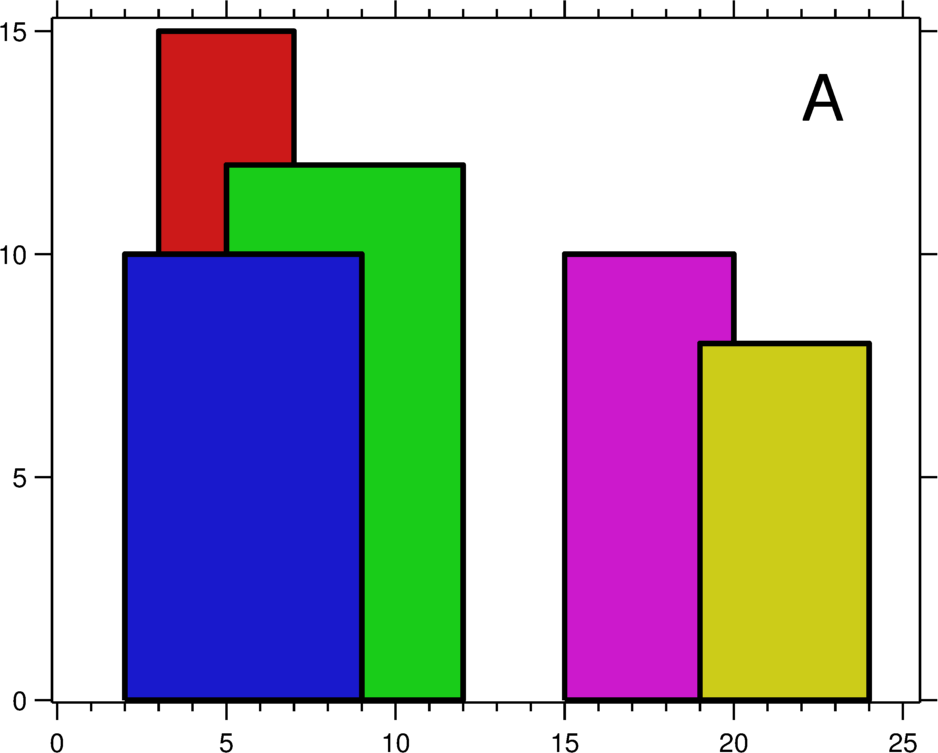
\includegraphics[width=150pt]{skyline1.png}
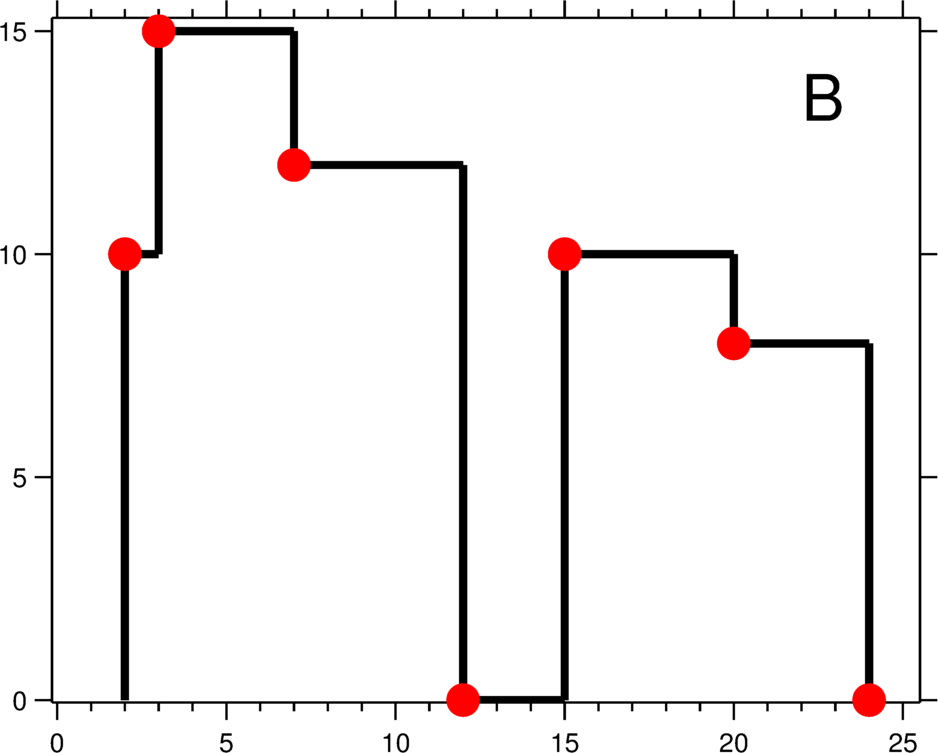
\includegraphics[width=150pt]{skyline2.png}
\end{center}

The geometric information of each building is represented by a triplet of integers [Li, Ri, Hi], where Li and Ri are the x coordinates of the left and right edge of the ith building, respectively, and Hi is its height. It is guaranteed that 0 ≤ Li, Ri ≤ INT_MAX, 0 < Hi ≤ INT_MAX, and Ri - Li > 0. You may assume all buildings are perfect rectangles grounded on an absolutely flat surface at height 0.

For instance, the dimensions of all buildings in Figure A are recorded as: [ [2 9 10], [3 7 15], [5 12 12], [15 20 10], [19 24 8] ] .

The output is a list of "key points" (red dots in Figure B) in the format of [ [x1,y1], [x2, y2], [x3, y3], ... ] that uniquely defines a skyline. A key point is the left endpoint of a horizontal line segment. Note that the last key point, where the rightmost building ends, is merely used to mark the termination of the skyline, and always has zero height. Also, the ground in between any two adjacent buildings should be considered part of the skyline contour.

For instance, the skyline in Figure B should be represented as:[ [2 10], [3 15], [7 12], [12 0], [15 10], [20 8], [24, 0] ].

\textbf{Notes:}

The number of buildings in any input list is guaranteed to be in the range [0, 10000].

The input list is already sorted in ascending order by the left x position Li.

The output list must be sorted by the x position.

There must be no consecutive horizontal lines of equal height in the output skyline. For instance, [...[2 3], [4 5], [7 5], [11 5], [12 7]...] is not acceptable; the three lines of height 5 should be merged into one in the final output as such: [...[2 3], [4 5], [12 7], ...]

\subsubsection{Analysis}

这题的核心就是求外轮廓,就是所有building覆盖到的区域的最高处构成的轮廓,所以我们关注的核心是当前有效区域的最高处,所以我们要维护一个大端队列,当在当前轮廓上碰到更高的矩形时,会生成一个新转折点,当当前轮廓所在的矩形结束时,轮廓高度会坠落到第二级台阶上。
每个building有两条竖线,左边为升,右边为降。我们遍历所有building,生成所有竖线的集合并排序,注意升线的高度设为负数。特殊情况:多条竖线重合,有升有降。我们优先看升,且优先看高度最高的升,因为会影响整个外轮廓
当矩形起始时,需要将其高度加入队列,如果其高度高于当前高度,则生成一个转折点,矩形结束时,需要将其高度从队列中去掉,如果结束点不在外轮廓上则不会生成转折点,就是说
即使去掉了该矩形的高度也不会影响队列中的最高高度,那外轮廓就不会变,不会有转折点。

\newpage

\subsubsection{Solution I}

\begin{Code}
// 耗时290ms,复杂度O(nlgn+nlgn+n^2)
public List<int[]> getSkyline(int[][] buildings) {
    List<int[]> heights = new LinkedList<int[]>();

    for (int[] building : buildings) {
        heights.add(new int[] {building[0], -building[2]});
        heights.add(new int[] {building[1], building[2]});
    }

    /**
     * 这里排序先按x,x相同则按高度,由于升线高度为负,所以升线越高越靠前,降线越矮越靠前。
     * x一定时升线高的靠前,因为决定最终结果的是升线最高的那个,如果不是这样,后面处理queue的时候会
     * 添加一堆中间结果x一定时降线矮的靠前,因为不这样的话,后面处理queue的时候会添加一堆中间结果
     */
    Collections.sort(heights, new Comparator<int[]>() {
        @Override
        public int compare(int[] o1, int[] o2) {
            return o1[0] == o2[0] ? o1[1] - o2[1] : o1[0] - o2[0];
        }
    });

    Queue<Integer> queue = new PriorityQueue<>(new Comparator<Integer>() {
        @Override
        public int compare(Integer o1, Integer o2) {
            return o2 - o1;
        }
    });

    /**
     * 这里别掉了
     */
    queue.offer(0);

    List<int[]> result = new LinkedList<int[]>();

    int prev = 0;
    for (int[] height : heights) {
        if (height[1] < 0) {
            queue.add(-height[1]);
        } else {
            queue.remove(height[1]);
        }
        int cur = queue.peek();
        if (prev != cur) {
            result.add(new int[] {height[0], cur});
            prev = cur;
        }
    }

    return result;
}
\end{Code}

\newpage

\subsubsection{Solution II}

\begin{Code}
/**
 * 上面PriorityQueue的remove复杂度为O(n),所以这里换成了TreeMap,删除的复杂度为O(lgn)
 */
// 耗时50ms,复杂度O(nlgn+nlgn+nlgn)
public List<int[]> getSkyline2(int[][] buildings) {
    List<int[]> heights = new LinkedList<int[]>();

    for (int[] building : buildings) {
        heights.add(new int[] {building[0], -building[2]});
        heights.add(new int[] {building[1], building[2]});
    }

    Collections.sort(heights, new Comparator<int[]>() {
        @Override
        public int compare(int[] o1, int[] o2) {
            return o1[0] == o2[0] ? o1[1] - o2[1] : o1[0] - o2[0];
        }
    });

    TreeMap<Integer, Integer> map = new TreeMap<>(Collections.<Integer>reverseOrder());

    // 这里一定别掉了
    map.put(0, 1);

    List<int[]> result = new LinkedList<int[]>();

    int prev = 0;
    for (int[] height : heights) {
        if (height[1] < 0) {
            map.put(-height[1], map.getOrDefault(-height[1], 0) + 1);
        } else {
            int cnt = map.getOrDefault(height[1], 0);
            if (cnt == 1) {
                map.remove(height[1]);
            } else {
                map.put(height[1], cnt - 1);
            }
        }
        int cur = map.firstKey();
        if (prev != cur) {
            result.add(new int[] {height[0], cur});
            prev = cur;
        }
    }

    return result;
}
\end{Code}

\newpage


\section{Top K Frequent Elements} %%%%%%%%%%%%%%%%%%%%%%



\subsubsection{Description}
Given a non-empty array of integers, return the k most frequent elements.

For example,

Given [1,1,1,2,2,3] and k = 2, return [1,2].

\textbf{Note:}

You may assume k is always valid, 1 ≤ k ≤ number of unique elements.

Your algorithm's time complexity must be better than O(n log n), where n is the array's size.

\subsubsection{Solution I}

\begin{Code}
// 耗时46ms,最差复杂度O(nlgn)
public List<Integer> topKFrequent(int[] nums, int k) {
    Map<Integer, Integer> map = new TreeMap<Integer, Integer>();
    for (int n : nums) {
        map.put(n, map.getOrDefault(n, 0) + 1);
    }
    Queue<int[]> queue = new PriorityQueue<>(new Comparator<int[]>() {
        @Override
        public int compare(int[] o1, int[] o2) {
            return o2[1] - o1[1];
        }
    });
    for (int key : map.keySet()) {
        queue.add(new int[] { key, map.get(key) });
    }
    List<Integer> list = new LinkedList<Integer>();
    for (int i = 1; i <= k && !queue.isEmpty(); i++) {
        list.add(queue.poll()[0]);
    }
    return list;
}
\end{Code}

\newpage

\subsubsection{Solution II}

\begin{Code}
// 耗时23ms,复杂度O(n)
public List<Integer> topKFrequent2(int[] nums, int k) {
    Map<Integer, Integer> map = new HashMap<Integer, Integer>();
    for (int n : nums) {
        map.put(n, map.getOrDefault(n, 0) + 1);
    }
    List<Integer>[] lists = new LinkedList[nums.length + 1];
    for (int key : map.keySet()) {
        int count = map.get(key);
        if (lists[count] == null) {
            lists[count] = new LinkedList<Integer>();
        }
        lists[count].add(key);
    }
    List<Integer> result = new LinkedList<Integer>();
    for (int i = lists.length - 1; i >= 0 && result.size() < k; i--) {
        if (lists[i] != null) {
            result.addAll(lists[i]);
        }
    }
    return result;
}
\end{Code}

\newpage

\section{Find Median from Data Stream} %%%%%%%%%%%%%%%%%%%%%%



\subsubsection{Description}
Median is the middle value in an ordered integer list. If the size of the list is even, there is no middle value. So the median is the mean of the two middle value.

\textbf{Examples:}

[2,3,4] , the median is 3

[2,3], the median is (2 + 3) / 2 = 2.5

Design a data structure that supports the following two operations:

void addNum(int num) - Add a integer number from the data stream to the data structure.
double findMedian() - Return the median of all elements so far.

For example:
\begin{Code}
addNum(1)
addNum(2)
findMedian() -> 1.5
addNum(3)
findMedian() -> 2
\end{Code}

\subsubsection{Solution}

\begin{Code}
/**
 * 比较大的一半
 */
PriorityQueue<Integer> maxheap = new PriorityQueue<Integer>();

/**
 * 比较小的一半
 */
PriorityQueue<Integer> minheap = new PriorityQueue<Integer>(Collections.reverseOrder());

// Adds a number into the data structure.
public void addNum(int num) {
    maxheap.offer(num);
    minheap.offer(maxheap.poll());

    /**
     * 要保证比较大的一半的size大于等于小的一半
     */
    if(maxheap.size() < minheap.size()){
        maxheap.offer(minheap.poll());
    }
}

// Returns the median of current data stream
public double findMedian() {
    return maxheap.size() == minheap.size() ?
        (double)(maxheap.peek() + minheap.peek()) / 2.0 : maxheap.peek();
}
\end{Code}

\newpage

\section{Kth Smallest Element in a Sorted Matrix} %%%%%%%%%%%%%%%%%%%%%%



\subsubsection{Description}
Given a n x n matrix where each of the rows and columns are sorted in ascending order, find the kth smallest element in the matrix.

Note that it is the kth smallest element in the sorted order, not the kth distinct element.

Example:

\begin{Code}
matrix = [
   [ 1,  5,  9],
   [10, 11, 13],
   [12, 13, 15]
],
k = 8,

return 13.
\end{Code}

\textbf{Note:}

You may assume k is always valid, 1 ≤ k ≤ n2.

\subsubsection{Solution}

\begin{Code}
public int kthSmallest(int[][] matrix, int k) {
    int n = matrix.length;
    PriorityQueue<Tuple> pq = new PriorityQueue<Tuple>();
    for(int j = 0; j <= n-1; j++) pq.offer(new Tuple(0, j, matrix[0][j]));
    for(int i = 0; i < k-1; i++) {
        Tuple t = pq.poll();
        if(t.x == n-1) continue;
        pq.offer(new Tuple(t.x+1, t.y, matrix[t.x+1][t.y]));
    }
    return pq.poll().val;
}

class Tuple implements Comparable<Tuple> {
    int x, y, val;
    public Tuple (int x, int y, int val) {
        this.x = x;
        this.y = y;
        this.val = val;
    }

    @Override
    public int compareTo (Tuple that) {
        return this.val - that.val;
    }
}
\end{Code}

\newpage

\section{Sort Characters By Frequency} %%%%%%%%%%%%%%%%%%%%%%



\subsubsection{Description}
Given a string, sort it in decreasing order based on the frequency of characters.

\textbf{Example 1:}

\textbf{Input:}

"tree"

\textbf{Output:}
"eert"

\textbf{}Explanation:

'e' appears twice while 'r' and 't' both appear once.

So 'e' must appear before both 'r' and 't'. Therefore "eetr" is also a valid answer.

\textbf{Example 2:}

\textbf{Input:}

"cccaaa"

\textbf{Output:}

"cccaaa"

\textbf{Explanation:}

Both 'c' and 'a' appear three times, so "aaaccc" is also a valid answer.

Note that "cacaca" is incorrect, as the same characters must be together.

\textbf{Example 3:}

\textbf{Input:}

"Aabb"

\textbf{Output:}

"bbAa"

\textbf{Explanation:}

"bbaA" is also a valid answer, but "Aabb" is incorrect.

Note that 'A' and 'a' are treated as two different characters.

\newpage

\subsubsection{Solution I}

\begin{Code}
public String frequencySort(String s) {
    Map<Character, Integer> map = new HashMap<>();
    for (char c : s.toCharArray()) {
        if (map.containsKey(c)) {
            map.put(c, map.get(c) + 1);
        } else {
            map.put(c, 1);
        }
    }
    List<Character> [] bucket = new List[s.length() + 1];
    for (char key : map.keySet()) {
        int frequency = map.get(key);
        if (bucket[frequency] == null) {
            bucket[frequency] = new ArrayList<>();
        }
        bucket[frequency].add(key);
    }
    StringBuilder sb = new StringBuilder();
    for (int pos = bucket.length - 1; pos >=0; pos--) {
        if (bucket[pos] != null) {
            for (char num : bucket[pos]) {
                for (int i = 0; i < map.get(num); i++) {
                    sb.append(num);
                }
            }
        }
    }
    return sb.toString();
}

\end{Code}

\newpage
\subsubsection{Solution II}

\begin{Code}
public String frequencySort(String s) {
    Map<Character, Integer> map = new HashMap<>();
    for (char c : s.toCharArray()) {
        if (map.containsKey(c)) {
            map.put(c, map.get(c) + 1);
        } else {
            map.put(c, 1);
        }
    }
    PriorityQueue<Map.Entry<Character, Integer>> pq = new PriorityQueue<>(
            new Comparator<Map.Entry<Character, Integer>>() {
                @Override
                public int compare(Map.Entry<Character, Integer> a, Map.Entry<Character, Integer> b) {
                    return b.getValue() - a.getValue();
                }
            }
    );
    pq.addAll(map.entrySet());
    StringBuilder sb = new StringBuilder();
    while (!pq.isEmpty()) {
        Map.Entry e = pq.poll();
        for (int i = 0; i < (int)e.getValue(); i++) {
            sb.append(e.getKey());
        }
    }
    return sb.toString();
}
\end{Code}

\newpage


\section{Super Ugly Number} %%%%%%%%%%%%%%%%%%%%%%



\subsubsection{Description}
Write a program to find the nth super ugly number.

Super ugly numbers are positive numbers whose all prime factors are in the given prime list primes of size k. For example, [1, 2, 4, 7, 8, 13, 14, 16, 19, 26, 28, 32] is the sequence of the first 12 super ugly numbers given primes = [2, 7, 13, 19] of size 4.

\textbf{Note:}
\begin{Code}
(1) 1 is a super ugly number for any given primes.
(2) The given numbers in primes are in ascending order.
(3) 0 < k ≤ 100, 0 < n ≤ 106, 0 < primes[i] < 1000.
(4) The nth super ugly number is guaranteed to fit in a 32-bit signed integer.
\end{Code}

\subsubsection{Solution I}

\begin{Code}
public int nthSuperUglyNumber(int n, int[] primes) {
    int[] ugly = new int[n];
    int[] idx = new int[primes.length];

    ugly[0] = 1;
    for (int i = 1; i < n; i++) {
        //find next
        ugly[i] = Integer.MAX_VALUE;
        for (int j = 0; j < primes.length; j++)
            ugly[i] = Math.min(ugly[i], primes[j] * ugly[idx[j]]);

        //slip duplicate
        for (int j = 0; j < primes.length; j++) {
            while (primes[j] * ugly[idx[j]] <= ugly[i]) idx[j]++;
        }
    }

    return ugly[n - 1];
}

\end{Code}

\newpage
\subsubsection{Solution II}
\begin{Code}
public int nthSuperUglyNumber2(int n, int[] primes) {
    int[] ugly = new int[n];
    int[] idx = new int[primes.length];
    int[] val = new int[primes.length];
    Arrays.fill(val, 1);

    int next = 1;
    for (int i = 0; i < n; i++) {
        ugly[i] = next;

        next = Integer.MAX_VALUE;
        for (int j = 0; j < primes.length; j++) {
            //skip duplicate and avoid extra multiplication
            if (val[j] == ugly[i]) val[j] = ugly[idx[j]++] * primes[j];
            //find next ugly number
            next = Math.min(next, val[j]);
        }
    }

    return ugly[n - 1];
}
\end{Code}

\newpage
\subsubsection{Solution III}

\begin{Code}
public int nthSuperUglyNumberHeap(int n, int[] primes) {
    int[] ugly = new int[n];

    PriorityQueue<Num> pq = new PriorityQueue<>();
    for (int i = 0; i < primes.length; i++) pq.add(new Num(primes[i], 1, primes[i]));
    ugly[0] = 1;

    for (int i = 1; i < n; i++) {
        ugly[i] = pq.peek().val;
        while (pq.peek().val == ugly[i]) {
            Num nxt = pq.poll();
            pq.add(new Num(nxt.p * ugly[nxt.idx], nxt.idx + 1, nxt.p));
        }
    }

    return ugly[n - 1];
}

private class Num implements Comparable<Num> {
    int val;
    int idx;
    int p;

    public Num(int val, int idx, int p) {
        this.val = val;
        this.idx = idx;
        this.p = p;
    }

    @Override
    public int compareTo(Num that) {
        return this.val - that.val;
    }
}
\end{Code}

\newpage

\section{Find K Pairs with Smallest Sums} %%%%%%%%%%%%%%%%%%%%%%



\subsubsection{Description}
You are given two integer arrays nums1 and nums2 sorted in ascending order and an integer k.

Define a pair (u,v) which consists of one element from the first array and one element from the second array.

Find the k pairs (u1,v1),(u2,v2) ...(uk,vk) with the smallest sums.

\textbf{Example 1:}
\begin{Code}
Given nums1 = [1,7,11], nums2 = [2,4,6],  k = 3

Return: [1,2],[1,4],[1,6]

The first 3 pairs are returned from the sequence:
[1,2],[1,4],[1,6],[7,2],[7,4],[11,2],[7,6],[11,4],[11,6]
\end{Code}

\textbf{Example 2:}
\begin{Code}
Given nums1 = [1,1,2], nums2 = [1,2,3],  k = 2

Return: [1,1],[1,1]

The first 2 pairs are returned from the sequence:
[1,1],[1,1],[1,2],[2,1],[1,2],[2,2],[1,3],[1,3],[2,3]
\end{Code}

\textbf{Example 3:}
\begin{Code}
Given nums1 = [1,2], nums2 = [3],  k = 3

Return: [1,3],[2,3]

All possible pairs are returned from the sequence:
[1,3],[2,3]
\end{Code}
\subsubsection{Solution}

\begin{Code}
public List<int[]> kSmallestPairs(int[] nums1, int[] nums2, int k) {
    PriorityQueue<int[]> que = new PriorityQueue<>((a, b) -> a[0] + a[1] - b[0] - b[1]);
    List<int[]> res = new ArrayList<>();
    if (nums1.length == 0 || nums2.length == 0 || k == 0) return res;
    for (int i = 0; i < nums1.length && i < k; i++) que.offer(new int[]{nums1[i], nums2[0], 0});
    while (k-- > 0 && !que.isEmpty()) {
        int[] cur = que.poll();
        res.add(new int[]{cur[0], cur[1]});
        if (cur[2] == nums2.length - 1) continue;
        que.offer(new int[]{cur[0], nums2[cur[2] + 1], cur[2] + 1});
    }
    return res;
}
\end{Code}

\newpage

\section{Largest Number} %%%%%%%%%%%%%%%%%%%%%%



\subsubsection{Description}
Given a list of non negative integers, arrange them such that they form the largest number.

For example, given [3, 30, 34, 5, 9], the largest formed number is 9534330.

\textbf{Note:} The result may be very large, so you need to return a string instead of an integer.

\subsubsection{Solution}

\begin{Code}
public String largestNumber(int[] nums) {
    String[] strs = new String[nums.length];
    for (int i = 0; i < nums.length; i++) {
        strs[i] = String.valueOf(nums[i]);
    }
    Arrays.sort(strs, new Comparator<String>() {
        @Override
        public int compare(String o1, String o2) {
            String s1 = o1 + o2;
            String s2 = o2 + o1;
            return s2.compareTo(s1);
        }
    });
    StringBuilder sb = new StringBuilder();
    for (String str : strs) {
        sb.append(str);
    }
    int i = 0;
    for ( ; i < sb.length() && sb.charAt(i) == '0'; i++);
    return i >= sb.length() ? "0" : sb.substring(i);
}
\end{Code}

\newpage

\section{Valid Anagram} %%%%%%%%%%%%%%%%%%%%%%



\subsubsection{Description}
Given two strings s and t, write a function to determine if t is an anagram of s.

For example,
\begin{Code}
s = "anagram", t = "nagaram", return true.
s = "rat", t = "car", return false.
\end{Code}

\textbf{Note:}

You may assume the string contains only lowercase alphabets.

\textbf{Follow up:}

What if the inputs contain unicode characters? How would you adapt your solution to such case?

\subsubsection{Solution I}

\begin{Code}
// 耗时6ms,时间复杂度O(n)
public boolean isAnagram(String s, String t) {
    if (s.length() != t.length()) {
        return false;
    }
    int[] count = new int[256];
    for (int i = 0; i < s.length(); i++) {
        count[s.charAt(i)]++;
        count[t.charAt(i)]--;
    }
    for (int i = 'a'; i <= 'z'; i++) {
        if (count[i] != 0) {
            return false;
        }
    }
    return true;
}
\end{Code}

\subsubsection{Solution II}
\begin{Code}
// 耗时6ms,时间复杂度O(nlgn)
public boolean isAnagram2(String s, String t) {
    char[] ss = s.toCharArray();
    Arrays.sort(ss);
    char[] tt = t.toCharArray();
    Arrays.sort(tt);
    return Arrays.equals(ss, tt);
}
\end{Code}

\newpage

\section{Maximum Gap} %%%%%%%%%%%%%%%%%%%%%%



\subsubsection{Description}
Given an unsorted array, find the maximum difference between the successive elements in its sorted form.

Try to solve it in linear time/space.

Return 0 if the array contains less than 2 elements.

You may assume all elements in the array are non-negative integers and fit in the 32-bit signed integer range.

\newpage
\subsubsection{Solution}

\begin{Code}
// 耗时5ms,木桶原理
public int maximumGap(int[] nums) {
    if (nums.length < 2) {
        return 0;
    }

    int min = Integer.MAX_VALUE, max = Integer.MIN_VALUE;
    /**
     * 首先找出数组中最大值和最小值
     */
    for (int n : nums) {
        min = Math.min(min, n);
        max = Math.max(max, n);
    }

    if (min == max) {
        return 0;
    }

    /**
     * 有len个数,则有len-1个间隙,这里算出平均每个桶的宽度,桶的个数是len-1
     */
    int gap = (int) Math.ceil((double) (max - min) / (nums.length - 1));
    int[] mins = new int[nums.length - 1], maxs = new int[nums.length - 1];

    Arrays.fill(mins, Integer.MAX_VALUE);
    Arrays.fill(maxs, Integer.MIN_VALUE);

    /**
     * 这里要统计落在每个桶内的最大值和最小值
     */
    for (int n : nums) {
        if (n == min || n == max) {
            continue;
        }
        /**
         * 先算出n所在的桶
         */
        int index = (n - min) / gap;
        mins[index] = Math.min(mins[index], n);
        maxs[index] = Math.max(maxs[index], n);
    }

    int last = min, maxGap = Integer.MIN_VALUE;
    for (int i = 0; i < nums.length - 1; i++) {
        if (mins[i] == Integer.MAX_VALUE) {
            continue;
        }
        maxGap = Math.max(maxGap, mins[i] - last);
        last = maxs[i];
    }
    maxGap = Math.max(maxGap, max - last);
    return maxGap;
}
\end{Code}

\newpage

\section{Intersection of Two Arrays} %%%%%%%%%%%%%%%%%%%%%%



\subsubsection{Description}
Given two arrays, write a function to compute their intersection.

\textbf{Example:}

Given nums1 = [1, 2, 2, 1], nums2 = [2, 2], return [2].

\textbf{Note:}

Each element in the result must be unique.

The result can be in any order.

\subsubsection{Solution I}

\begin{Code}
public int[] intersection(int[] nums1, int[] nums2) {
    Set<Integer> set = new HashSet<>();
    Set<Integer> intersect = new HashSet<>();
    for (int i = 0; i < nums1.length; i++) {
        set.add(nums1[i]);
    }
    for (int i = 0; i < nums2.length; i++) {
        if (set.contains(nums2[i])) {
            intersect.add(nums2[i]);
        }
    }
    int[] result = new int[intersect.size()];
    int i = 0;
    for (Integer num : intersect) {
        result[i++] = num;
    }
    return result;
}
\end{Code}

\newpage

\subsubsection{Solution II}
\begin{Code}
public int[] intersection2(int[] nums1, int[] nums2) {
    Set<Integer> set = new HashSet<>();
    Arrays.sort(nums1);
    Arrays.sort(nums2);
    int i = 0;
    int j = 0;
    while (i < nums1.length && j < nums2.length) {
        if (nums1[i] < nums2[j]) {
            i++;
        } else if (nums1[i] > nums2[j]) {
            j++;
        } else {
            set.add(nums1[i]);
            i++;
            j++;
        }
    }
    int[] result = new int[set.size()];
    int k = 0;
    for (Integer num : set) {
        result[k++] = num;
    }
    return result;
}
\end{Code}

\newpage
\subsubsection{Solution III}
\begin{Code}
public int[] intersection3(int[] nums1, int[] nums2) {
    Set<Integer> set = new HashSet<>();
    Arrays.sort(nums2);
    for (Integer num : nums1) {
        if (binarySearch(nums2, num)) {
            set.add(num);
        }
    }
    int i = 0;
    int[] result = new int[set.size()];
    for (Integer num : set) {
        result[i++] = num;
    }
    return result;
}

public boolean binarySearch(int[] nums, int target) {
    int low = 0;
    int high = nums.length - 1;
    while (low <= high) {
        int mid = low + (high - low) / 2;
        if (nums[mid] == target) {
            return true;
        }
        if (nums[mid] > target) {
            high = mid - 1;
        } else {
            low = mid + 1;
        }
    }
    return false;
}
\end{Code}

\newpage

\section{Intersection of Two Arrays II} %%%%%%%%%%%%%%%%%%%%%%



\subsubsection{Description}
Given two arrays, write a function to compute their intersection.

\textbf{Example:}

Given nums1 = [1, 2, 2, 1], nums2 = [2, 2], return [2, 2].

\textbf{Note:}

Each element in the result should appear as many times as it shows in both arrays.

The result can be in any order.

\textbf{Follow up:}

What if the given array is already sorted? How would you optimize your algorithm?

What if nums1's size is small compared to nums2's size? Which algorithm is better?

What if elements of nums2 are stored on disk, and the memory is limited such that you cannot load all elements into the memory at once?
\subsubsection{Solution}

\begin{Code}
public int[] intersect(int[] nums1, int[] nums2) {
    HashMap<Integer, Integer> map = new HashMap<Integer, Integer>();
    ArrayList<Integer> result = new ArrayList<Integer>();
    for(int i = 0; i < nums1.length; i++)
    {
        if(map.containsKey(nums1[i])) map.put(nums1[i], map.get(nums1[i])+1);
        else map.put(nums1[i], 1);
    }

    for(int i = 0; i < nums2.length; i++)
    {
        if(map.containsKey(nums2[i]) && map.get(nums2[i]) > 0)
        {
            result.add(nums2[i]);
            map.put(nums2[i], map.get(nums2[i])-1);
        }
    }

    int[] r = new int[result.size()];
    for(int i = 0; i < result.size(); i++)
    {
        r[i] = result.get(i);
    }

    return r;
}
\end{Code}

\newpage

\section{Sort Colors} %%%%%%%%%%%%%%%%%%%%%%



\subsubsection{Description}
Given an array with n objects colored red, white or blue, sort them so that objects of the same color are adjacent, with the colors in the order red, white and blue.

Here, we will use the integers 0, 1, and 2 to represent the color red, white, and blue respectively.

\textbf{Note:}

You are not suppose to use the library's sort function for this problem.

\textbf{Follow up:}

A rather straight forward solution is a two-pass algorithm using counting sort.

First, iterate the array counting number of 0's, 1's, and 2's, then overwrite array with total number of 0's, then 1's and followed by 2's.

Could you come up with an one-pass algorithm using only constant space?

\subsubsection{Solution I}

\begin{Code}
/**
 * 从左往右遍历,如果遇到0,左边肯定先是一堆0,然后是1堆1,交换过后,当前肯定是1,所以要i++。
 * 如果遇到2,肯定往右交换,然后交换后的数未知,所以i不能轻举妄动
 */
// 时间复杂度O(n),扫一遍
public void sortColors3(int[] nums) {
    int zero = -1, two = nums.length;
    for (int i = 0; i < two; ) {
        if (nums[i] == 0) {
            swap(nums, ++zero, i++);
        } else if (nums[i] == 2) {
            swap(nums, --two, i);
        } else {
            i++;
        }
    }
}

private void swap(int[] nums, int i, int j) {
    int k = nums[i];
    nums[i] = nums[j];
    nums[j] = k;
}
\end{Code}

\newpage
\subsubsection{Solution II}
\begin{Code}
/**
 * 如果要扩展到k个颜色,如果颜色为0~k
 * 原理很简单,就是统计每个颜色的个数,转成负数,保存在原来的数组中
 * 统计完后再根据个数设置数组
 * 其实可以另外开辟一个数组保存个数,如果对空间没有要求的话
 */
public void sortKColors(int[] colors, int k) {
    for (int i = 0; i < colors.length; i++) {
        while (colors[i] >= 0) {
            int color = colors[i];
            if (colors[color] >= 0) {
                colors[i] = colors[color];
                colors[color] = -2;
            } else {
                colors[color]--;
                colors[i] = -1;
            }
        }
    }
    for (int i = colors.length - 1; i >= 0; ) {
        int color = --k, count = -(colors[color] + 1);
        for (int j = 0; j < count; j++) {
            colors[i--] = color;
        }
    }
}
\end{Code}

\subsubsection{Solution III}
\begin{Code}
/**
 * http://www.lintcode.com/zh-cn/problem/sort-colors-ii/
 */
// 如果颜色从1~k,lint
public void sortColors2(int[] colors, int k) {
    // write your code here
    for (int i = 0; i < colors.length; i++) {
        while (colors[i] > 0) {
            int color = colors[i];
            if (colors[color - 1] > 0) {
                colors[i] = colors[color - 1];
                colors[color - 1] = -1;
            } else {
                colors[color - 1]--;
                colors[i] = 0;
            }
        }
    }
    int color = k - 1;
    for (int i = colors.length - 1; i >= 0; ) {
        for (int j = 0; j < -colors[color]; j++) {
            colors[i--] = color + 1;
        }
        color--;
    }
}

\end{Code}

\newpage

\section{Wiggle Sort} %%%%%%%%%%%%%%%%%%%%%%



\subsubsection{Description}
Given an unsorted array nums, reorder it in-place such that nums[0] <= nums[1] >= nums[2] <= nums[3]....

For example, given nums = \code{[3, 5, 2, 1, 6, 4]}, one possible answer is \code{[1, 6, 2, 5, 3, 4]}.

\subsubsection{Solution I}

\begin{Code}
public void wiggleSort(int[] nums) {
    Arrays.sort(nums);
    for (int i = 1; i + 1 < nums.length; i += 2) {
        swap(nums, i, i + 1);
    }
}
\end{Code}

\subsubsection{Solution II}
\begin{Code}
// 复杂度O(n)
public void wiggleSort2(int[] nums) {
    for (int i = 0; i + 1 < nums.length; i++) {
        if ((i & 1) == 0) {
            if (nums[i] > nums[i + 1]) {
                swap(nums, i, i + 1);
            }
        } else {
            if (nums[i] < nums[i + 1]) {
                swap(nums, i, i + 1);
            }
        }
    }
}

private void swap(int[] nums, int i, int j) {
    int t = nums[i];
    nums[i] = nums[j];
    nums[j] = t;
}

\end{Code}

\newpage

\section{Wiggle Sort II} %%%%%%%%%%%%%%%%%%%%%%



\subsubsection{Description}
Given an unsorted array nums, reorder it such that nums[0] < nums[1] > nums[2] < nums[3]....

\textbf{Example:}
\begin{Code}
(1) Given nums = [1, 5, 1, 1, 6, 4], one possible answer is [1, 4, 1, 5, 1, 6].
(2) Given nums = [1, 3, 2, 2, 3, 1], one possible answer is [2, 3, 1, 3, 1, 2].
\end{Code}

\textbf{Note:}

You may assume all input has valid answer.

\textbf{Follow Up:}

Can you do it in O(n) time and/or in-place with O(1) extra space?

\subsubsection{Solution I}

\begin{Code}
// 时间复杂度O(nlgn),空间复杂度O(n)
public void wiggleSort2(int[] nums) {
    int[] arr = nums.clone();
    Arrays.sort(arr);
    int n = nums.length, k = (n - 1) / 2, j = n - 1;
    for (int i = 0; i < n; i++) {
        nums[i] = (i & 1) != 0 ? arr[j--] : arr[k--];
    }
}
\end{Code}

\subsubsection{Solution II}
\begin{Code}
/**
 * 这个更优解法没看明白
 */
// 时间复杂度O(n),空间复杂度O(l)
public void wiggleSort(int[] nums) {
    int len = nums.length;
    int median = findKthLargest(nums, (len + 1) / 2);
    for (int left = 0, right = len - 1, i = 0; i <= right; ) {
        if (nums[newIndex(i, len)] > median) {
            swap(nums, newIndex(left++, len), newIndex(i++, len));
        } else if (nums[newIndex(i, len)] < median) {
            swap(nums, newIndex(right--, len), newIndex(i, len));
        } else {
            i++;
        }
    }
}

private int newIndex(int index, int n) {
    return (1 + 2 * index) % (n | 1);
}

private void swap(int[] nums, int i, int j) {
    int t = nums[i];
    nums[i] = nums[j];
    nums[j] = t;
}

public int findKthLargest(int[] nums, int k) {
    return nums[findKthLargest(nums, 0, nums.length - 1, k)];
}

public int findKthLargest(int[] nums, int start, int end, int k) {
    int pivot = partition(nums, start, end);

    int rank = end - pivot + 1;

    if (rank == k) {
        return pivot;
    } else if (rank > k) {
        return findKthLargest(nums, pivot + 1, end, k);
    } else {
        return findKthLargest(nums, start, pivot - 1, k - rank);
    }
}

public int partition(int[] nums, int start, int end) {
    int pivot = nums[end], left = start;

    for (int i = start; i < end; i++) {
        if (nums[i] <= pivot) {
            swap(nums, left++, i);
        }
    }

    swap(nums, left, end);

    return left;
}
\end{Code}

\newpage

\section{H-Index} %%%%%%%%%%%%%%%%%%%%%%



\subsubsection{Description}
Given an array of citations (each citation is a non-negative integer) of a researcher, write a function to compute the researcher's h-index.

According to the definition of h-index on Wikipedia: "A scientist has index h if h of his/her N papers have at least h citations each, and the other N − h papers have no more than h citations each."

For example, given citations = [3, 0, 6, 1, 5], which means the researcher has 5 papers in total and each of them had received 3, 0, 6, 1, 5 citations respectively. Since the researcher has 3 papers with at least 3 citations each and the remaining two with no more than 3 citations each, his h-index is 3.

\textbf{Note:} If there are several possible values for h, the maximum one is taken as the h-index.

\subsubsection{Solution I}

\begin{Code}
// 耗时4ms,时间复杂度O(nlgn)
public int hIndex(int[] citations) {
    Arrays.sort(citations);
    int hIndex = 0;
    for (int i = citations.length - 1; i >= 0; i--) {
        hIndex = Math.max(hIndex, Math.min(citations.length - i, citations[i]));
    }
    return hIndex;
}
\end{Code}

\subsubsection{Solution II}
\begin{Code}
// 耗时1ms,时间复杂度O(n)
public int hIndex2(int[] citations) {
    /**
     * 大于文章数的引用可以合并到一起
     */
    int n = citations.length;
    int[] f = new int[n + 1];
    for (int k : citations) {
        f[Math.min(k, n)]++;
    }
    int hindex = 0;
    /**
     * i表示引用数,j表示大于等于该引用数的总文章数
     */
    for (int i = n, j = 0; i >= 0; i--) {
        j += f[i];
        hindex = Math.max(hindex, Math.min(j, i));
    }
    return hindex;
}

\end{Code}

\newpage

\section{H-Index II} %%%%%%%%%%%%%%%%%%%%%%



\subsubsection{Description}
Follow up for H-Index: What if the citations array is sorted in ascending order? Could you optimize your algorithm?

\subsubsection{Solution}

\begin{Code}
public int hIndex(int[] citations) {
    int len = citations.length, left = 0, right = len - 1;

    while (left <= right) {
        int mid = left + ((right - left) >>> 1);

        int articles = len - mid;

        if (articles == citations[mid]) {
            // 这是临界点,再往下文章数会大于引用
            return articles;
        } else if (articles > citations[mid]) {
            // 文章数大于引用,继续往下走
            left = mid + 1;
        } else {
            // 文章数小于引用,继续往前走
            right = mid - 1;
        }
    }

    return len - left;
}
\end{Code}

\newpage

\section{Guess Number Higher or Lower} %%%%%%%%%%%%%%%%%%%%%%



\subsubsection{Description}
We are playing the Guess Game. The game is as follows:

I pick a number from 1 to n. You have to guess which number I picked.

Every time you guess wrong, I'll tell you whether the number is higher or lower.

You call a pre-defined API guess(int num) which returns 3 possible results (-1, 1, or 0):
\begin{Code}
-1 : My number is lower
 1 : My number is higher
 0 : Congrats! You got it!
\end{Code}

\textbf{Example:}

n = 10, I pick 6.

Return 6.

\subsubsection{Solution}

\begin{Code}
public int guessNumber(int n) {
    int left = 1, right = n;

    while (left < right) {
        int mid = left + ((right - left) >>> 1);

        int guess = guess(mid);

        if (guess > 0) {
            left = mid + 1;
        } else if (guess < 0) {
            right = mid - 1;
        } else {
            return mid;
        }
    }

    return left;
}
\end{Code}

\newpage

\section{First Bad Version} %%%%%%%%%%%%%%%%%%%%%%



\subsubsection{Description}
You are a product manager and currently leading a team to develop a new product. Unfortunately, the latest version of your product fails the quality check. Since each version is developed based on the previous version, all the versions after a bad version are also bad.

Suppose you have n versions [1, 2, ..., n] and you want to find out the first bad one, which causes all the following ones to be bad.

You are given an API bool isBadVersion(version) which will return whether version is bad. Implement a function to find the first bad version. You should minimize the number of calls to the API.

\subsubsection{Solution I}

\begin{Code}
public int firstBadVersion(int n) {
    int left = 1, right = n;

    while (left < right) {
        int mid = left + ((right - left) >>> 1);

        if (isBadVersion(mid)) {
            right = mid;
        } else {
            left = mid + 1;
        }
    }

    return left;
}
\end{Code}

\subsubsection{Solution II}
\begin{Code}
public int firstBadVersion2(int n) {
    int left = 1, right = n;

    while (left <= right) {
        int mid = left + ((right - left) >> 1);

        if (isBadVersion(mid)) {
            right = mid - 1;
        } else {
            left = mid + 1;
        }
    }

    return left;
}
\end{Code}

\newpage

\section{4Sum} %%%%%%%%%%%%%%%%%%%%%%



\subsubsection{Description}
Given an array S of n integers, are there elements a, b, c, and d in S such that a + b + c + d = target? Find all unique quadruplets in the array which gives the sum of target.

Note: The solution set must not contain duplicate quadruplets.

For example, given array S = [1, 0, -1, 0, -2, 2], and target = 0.

A solution set is:
\begin{Code}
[
  [-1,  0, 0, 1],
  [-2, -1, 1, 2],
  [-2,  0, 0, 2]
]
\end{Code}
\subsubsection{Solution}

\begin{Code}
public List<List<Integer>> fourSum(int[] nums, int target) {
    Arrays.sort(nums);

    List<List<Integer>> result = new LinkedList<>();

    for (int i = 0; i + 3 < nums.length; i++) {
        if (i > 0 && nums[i] == nums[i - 1]) {
            continue;
        }

        for (int j = i + 1; j + 2 < nums.length; j++) {
            if (j != i + 1 && nums[j] == nums[j - 1]) {
                continue;
            }

            long newTarget = target - nums[i] - nums[j];
            for (int k = j + 1, m = nums.length - 1; k < m; ) {
                long sum = nums[k] + nums[m];
                if (sum > newTarget) {
                    m--;
                } else if (sum < newTarget) {
                    k++;
                } else {
                    result.add(Arrays.asList(nums[i], nums[j], nums[k], nums[m]));

                    k++, m--;
                    for ( ; k < m && nums[k] == nums[k - 1] && nums[m] == nums[m + 1]; k++, m--);
                }
            }
        }
    }

    return result;
}
\end{Code}

\newpage

\section{Valid Perfect Square} %%%%%%%%%%%%%%%%%%%%%%



\subsubsection{Description}
Given a positive integer num, write a function which returns True if num is a perfect square else False.

\textbf{Note:} Do not use any built-in library function such as sqrt.

\textbf{Example 1:}

\textbf{Input:} 16

\textbf{Returns:} True

\textbf{Example 2:}

\textbf{Input:} 14

\textbf{Returns:} False
\subsubsection{Solution I}

\begin{Code}
public boolean isPerfectSquare(int num) {
    int i = 1;
    while (num > 0) {
        num -= i;
        i += 2;
    }
    return num == 0;
}
\end{Code}

\subsubsection{Solution II}
\begin{Code}
public boolean isPerfectSquare2(int num) {
    int low = 1, high = num;
    while (low <= high) {
        long mid = (low + high) >>> 1;
        if (mid * mid == num) {
            return true;
        } else if (mid * mid < num) {
            low = (int) mid + 1;
        } else {
            high = (int) mid - 1;
        }
    }
    return false;
}
\end{Code}
\subsubsection{Solution III}
\begin{Code}
public boolean isPerfectSquare3(int num) {
    long x = num;
    while (x * x > num) {
        x = (x + num / x) >> 1;
    }
    return x * x == num;
}
\end{Code}

\newpage

\section{Smallest Rectangle Enclosing Black Pixels} %%%%%%%%%%%%%%%%%%%%%%



\subsubsection{Description}
An image is represented by a binary matrix with 0 as a white pixel and 1 as a black pixel. The black pixels are connected, i.e., there is only one black region. Pixels are connected horizontally and vertically. Given the location (x, y) of one of the black pixels, return the area of the smallest (axis-aligned) rectangle that encloses all black pixels.

For example, given the following image:
\begin{Code}
[
  "0010",
  "0110",
  "0100"
]
\end{Code}

and x = 0, y = 2,

Return 6.
\subsubsection{Solution}

\begin{Code}
private char[][] image;

public int minArea(char[][] iImage, int x, int y) {
    image = iImage;
    int m = image.length, n = image[0].length;
    int left = searchColumns(0, y, 0, m, true);
    int right = searchColumns(y + 1, n, 0, m, false);
    int top = searchRows(0, x, left, right, true);
    int bottom = searchRows(x + 1, m, left, right, false);
    return (right - left) * (bottom - top);
}

private int searchColumns(int i, int j, int top, int bottom, boolean opt) {
    while (i != j) {
        int k = top, mid = (i + j) / 2;
        while (k < bottom && image[k][mid] == '0') ++k;
        if (k < bottom == opt)
            j = mid;
        else
            i = mid + 1;
    }
    return i;
}

private int searchRows(int i, int j, int left, int right, boolean opt) {
    while (i != j) {
        int k = left, mid = (i + j) / 2;
        while (k < right && image[mid][k] == '0') ++k;
        if (k < right == opt)
            j = mid;
        else
            i = mid + 1;
    }
    return i;
}
\end{Code}

\newpage

\section{Smallest Good Base} %%%%%%%%%%%%%%%%%%%%%%



\subsubsection{Description}
For an integer n, we call k>=2 a good base of n, if all digits of n base k are 1.

Now given a string representing n, you should return the smallest good base of n in string format.

\textbf{Example 1:}

\textbf{Input:} "13"

\textbf{Output:} "3"

\textbf{Explanation:} 13 base 3 is 111.

\textbf{Example 2:}

\textbf{Input:} "4681"

\textbf{Output:} "8"

\textbf{Explanation:} 4681 base 8 is 11111.

\textbf{Example 3:}

\textbf{Input:} "1000000000000000000"

\textbf{Output:} "999999999999999999"

\textbf{Explanation:} 1000000000000000000 base 999999999999999999 is 11.

\textbf{Note:}

The string representing n is always valid and will not have leading zeros.
\subsubsection{Solution}

\begin{Code}
public String smallestGoodBase(String nn) {
    long n = Long.parseLong(nn);
    long res = 0;
    for (int k = 60; k >= 2; k--) {
        long s = 2, e = n;
        while (s < e) {
            long m = s + (e - s) / 2;
            BigInteger left = BigInteger.valueOf(m);
            left = left.pow(k).subtract(BigInteger.ONE);
            BitInteger temp = BigInteger.valueOf(m).subtract(BigInteger.ONE);
            BigInteger right = BigInteger.valueOf(n).multiply(temp);
            int cmr = left.compareTo(right);
            if (cmr == 0) {
                res = m;
                break;
            } else if (cmr < 0) {
                s = m + 1;
            } else {
                e = m;
            }
        }
        if (res != 0) break;
    }
    return "" + res;
}
\end{Code}

\newpage

\section{Find Right Interval} %%%%%%%%%%%%%%%%%%%%%%



\subsubsection{Description}
Given a set of intervals, for each of the interval i, check if there exists an interval j whose start point is bigger than or equal to the end point of the interval i, which can be called that j is on the "right" of i.

For any interval i, you need to store the minimum interval j's index, which means that the interval j has the minimum start point to build the "right" relationship for interval i. If the interval j doesn't exist, store -1 for the interval i. Finally, you need output the stored value of each interval as an array.

\textbf{Note:}

You may assume the interval's end point is always bigger than its start point.

You may assume none of these intervals have the same start point.

\textbf{Example 1:}

\textbf{Input:} [ [1,2] ]

\textbf{Output:} [-1]

\textbf{Explanation:} There is only one interval in the collection, so it outputs -1.

\textbf{Example 2:}

\textbf{Input:} [ [3,4], [2,3], [1,2] ]

\textbf{Output:} [-1, 0, 1]

\textbf{Explanation:} There is no satisfied "right" interval for [3,4].

For [2,3], the interval [3,4] has minimum-"right" start point;

For [1,2], the interval [2,3] has minimum-"right" start point.

\textbf{Example 3:}

\textbf{Input:} [ [1,4], [2,3], [3,4] ]

\textbf{Output:} [-1, 2, -1]

\textbf{Explanation:} There is no satisfied "right" interval for [1,4] and [3,4].

For [2,3], the interval [3,4] has minimum-"right" start point.

\subsubsection{Solution}

\begin{Code}
public int[] findRightInterval(Interval[] intervals) {
    int[] result = new int[intervals.length];
    java.util.NavigableMap<Integer, Integer> intervalMap = new TreeMap<>();

    for (int i = 0; i < intervals.length; ++i) {
        intervalMap.put(intervals[i].start, i);
    }

    for (int i = 0; i < intervals.length; ++i) {
        Map.Entry<Integer, Integer> entry = intervalMap.ceilingEntry(intervals[i].end);
        result[i] = (entry != null) ? entry.getValue() : -1;
    }

    return result;
}
\end{Code}